\documentclass[11pt, oneside]{article}
\usepackage{geometry}
\geometry{letterpaper}
\usepackage{graphicx}
\usepackage{amssymb}
\usepackage{wrapfig}

\title{Usability Metrics and Heuristic Analysis of iOS Reading Applications}
\author{Adrian Lu}
\date{\today}

\begin{document}
\maketitle

\section{Introduction}
For our usability survey, we decided to test different iOS reading applications. The applications we chose to compare were iBooks by Apple, and Kindle by Amazon. To quantify the usability of these applications, we are going to measure learnability, errors, and satisfaction. Learnability will be tested temporally, errors will be measured upon the number of errors made, and satisfaction should have been quantified on a numerical scale from 1 to 10, however in our tests we asked for comments on the process instead of a numerical response. The three tasks that we gave said subjects were as follows:

\begin{enumerate}
    \item Finding, and subsequently downloading, a predetermined eBook from the various storefronts for the respective apps
    \item Highlighting and making a note/comment regarding the highlighted text
    \item Finding a predetermined passage from the book
\end{enumerate}

\section{Tests}

\subsection{Find and download a given book from Amazon and Apple}
For iBooks, testers were started on the iBooks app homepage, and were told to find and download \textit{Thrill} by Lucia Jordan. For Kindle, testers were started with a blank Safari web browser page, and given the same instructions. Note that due to Apple's in-app purchase policy, Amazon's Kindle app does not support in-app purchases, forcing users to buy books from Amazon.com, and then open the books up in the Kindle app.

\subsection{Highlight any passage from the book, and make an annotation}
For both platforms, users were started on the cover page of the book and were told to find any bit of text, and then both highlight it and make an annotation. Note that in iBooks, making an annotation automatically highlights the portion of text that you were annotating, while in Kindle, the actions are handled separately.

\subsection{Find a given quote within the book}
For both platforms, users were started again on the cover page of the book, and told to search for the following quote in the book: "Brandon Maxwell was no ordinary man." Note that in iBooks, the search button is displayed on the screen if the screen is tapped while reading, and in Kindle, the search function can only be reached after hitting a menu button that is shown when the screen is tapped.

%ALu: Dondi I tried so damn hard to get these sections to stop overlapping and preventing what is currently wrong with pages 3 and 4, but I cant for the life of me figure out how to get it to stop positioning these sections like it is. I feel like it should finish all the content held within 1 section before moving onto another, but it doesn't, and adding line breaks, page breaks, horizontal spaces all did nothing. Sorry I couldn't figure this out.

\section{Data Tables}

\begin{table}[!hbt]
% Center the table
\begin{center}
% Title of the table
\caption{Find/Download Book; iBooks}
\label{tab:task3learnKindle}
% Table itself: here we have two columns which are centered and have lines to the left, right and in the middle: |c|c|
\begin{tabular}{|c|c|c|c|}
% To create a horizontal line, type \hline
\hline
% To end a column type &
% For a linebreak type \\
$User$ & $Time$ $(sec)$ & $Errors$ & $Comments$\\
\hline
Albert & 22 & 1 & "Thrilling; Fantastic"\\
\hline
Alex & 17 & 0 & "Easy; Search could have auto-filled"\\
\hline
Andrew & 18 & 0 & "Easy"\\
\hline
Eko & 19 & 0 & "Search didn't give live results"\\
\hline
Harris & 30 & 0 & "Easy; Liked easy access download button"\\
\hline
Josh & 20 & 1 & "Easy; Paid options were on top"\\
\hline
Julia & 14 & 0 & "Easy; Similar to other iOS searches"\\
\hline
Justin & 17 & 0 & "Simple and intuitive"\\
\hline
Lauren & 10 & 0 & "Liked easy access download button"\\
\hline
Maurice & 35 & 1 & "Easy enough"\\
\hline
Ronald & 23 & 1 & "Not bad; Felt straightforward"\\
\hline
Sam & 28 & 1 & "Easy"\\
\hline
Tori & 18 & 1 & "Didn't live search; Fairly easy"\\
\hline
\end{tabular}
\end{center}
\end{table}

\begin{table}[!hbt]
% Center the table
\begin{center}
% Title of the table
\caption{Find/Download Book; Kindle}
\label{tab:task3learnKindle}
% Table itself: here we have two columns which are centered and have lines to the left, right and in the middle: |c|c|
\begin{tabular}{|c|c|c|c|}
% To create a horizontal line, type \hline
\hline
% To end a column type &
% For a linebreak type \\
$User$ & $Time$ $(sec)$ & $Errors$ & $Comments$\\
\hline
Albert & 20 & 0 & "Stupid to use the browser"\\
\hline
Alex & 21 & 0 & "Annoying to use browser"\\
\hline
Andrew & 18 & 0 & "Annoyed to use browser"\\
\hline
Eko & 15 & 0 & "iBooks didn't require Safari"\\
\hline
Harris & 125 & 1 & "Dumb; Frustrating; Used the ad results on Google"\\
\hline
Josh & 13 & 0 & "Used Google to find the book"\\
\hline
Julia & 18 & 0 & "Same basic process; No struggles"\\
\hline
Justin & 26 & 0 & "Was okay"\\
\hline
Lauren & 19 & 0 & "Liked the book"\\
\hline
Maurice & 34 & 0 & "Inferior because you couldn't do it in the app"\\
\hline
Ronald & 24 & 0 & "Really stupid"\\
\hline
Sam & 15 & 0 & "Easy but inconvenient"\\
\hline
Tori & 14 & 0 & "Too inconvenient"\\
\hline
\end{tabular}
\end{center}
\end{table}

\begin{table}[!hbt]
% Center the table
\begin{center}
% Title of the table
\caption{Highlight/Annotate; iBooks}
\label{tab:task3learnKindle}
% Table itself: here we have two columns which are centered and have lines to the left, right and in the middle: |c|c|
\begin{tabular}{|c|c|c|c|}
% To create a horizontal line, type \hline
\hline
% To end a column type &
% For a linebreak type \\
$User$ & $Time$ $(sec)$ & $Errors$ & $Comments$\\
\hline
Albert & 180 & 3 & "Unfortunate; Felt unnatural"\\
\hline
Alex & 6 & 0 & "Similar to Google Books"\\
\hline
Andrew & 15 & 0 & "Fairly okay"\\
\hline
Eko & 10 & 0 & "Felt very fulfilled"\\
\hline
Harris & 15 & 0 & "Intuitive"\\
\hline
Josh & 20 & 0 & "Took a few seconds to figure out where to go"\\
\hline
Julia & 38 & 1(?) & "Really frustrating; Didn't follow iOS convention"\\
\hline
Justin & 39 & 1 & "Not intuitive"\\
\hline
Lauren & 9 & 0 & "Not as easy as expected"\\
\hline
Maurice & 21 & 0 & "Pleasant enough"\\
\hline
Ronald & 15 & 0 & "Not bad; Fairly apparent"\\
\hline
Sam & 41 & 1(?) & "Hard and misleading"\\%made the same error repeatedly, hit the same button over and over expecting it to do something
\hline
Tori & 16 & 0 & "Very easy"\\
\hline
\end{tabular}
\end{center}
\end{table}

\begin{table}[!hbt]
% Center the table
\begin{center}
% Title of the table
\caption{Highlight/Annotate; Kindle}
\label{tab:task3learnKindle}
% Table itself: here we have two columns which are centered and have lines to the left, right and in the middle: |c|c|
\begin{tabular}{|c|c|c|c|}
% To create a horizontal line, type \hline
\hline
% To end a column type &
% For a linebreak type \\
$User$ & $Time$ $(sec)$ & $Errors$ & $Comments$\\
\hline
Albert & 17 & 1 & "Instinctual"\\
\hline
Alex & 13 & 0 & "Encountered a bug in the app"\\
\hline
Andrew & 27 & 1 & "Physical Kindle highlights when a note is made"\\
\hline
Eko & 13 & 0 & "This is hard"\\
\hline
Harris & 15 & 1 & "It was alright; Not the most intuitive"\\
\hline
Josh & 19 & 0 & "Liked choosing a highlighting color"\\
\hline
Julia & 18 & 0 & "Easy"\\
\hline
Justin & 19 & 1 & "Very similar; Didn't highlight annotation"\\
\hline
Lauren & 6 & 0 & "Some of the icons looked very similar"\\
\hline
Maurice & 19 & 0 & "Felt unnatural"\\
\hline
Ronald & 20 & 0 & "Pretty similar to other iOS functions"\\
\hline
Sam & 14 & 0 & "Icons felt hidden"\\
\hline
Tori & 13 & 0 & "Highlight colors were great"\\
\hline
\end{tabular}
\end{center}
\end{table}

\begin{table}[!hbt]
% Center the table
\begin{center}
% Title of the table
\caption{Find Quote; iBooks}
\label{tab:task3learnKindle}
% Table itself: here we have two columns which are centered and have lines to the left, right and in the middle: |c|c|
\begin{tabular}{|c|c|c|c|}
% To create a horizontal line, type \hline
\hline
% To end a column type &
% For a linebreak type \\
$User$ & $Time$ $(sec)$ & $Errors$ & $Comments$\\
\hline
Albert & 24 & 0 & "Worthwhile; Ordinary"\\
\hline
Alex & 12 & 0 & "Keyboard issues"\\
\hline
Andrew & 16 & 0 & "Did what was expected"\\
\hline
Eko & 11 & 0 & "Search was intuitive"\\
\hline
Harris & 12 & 0 & "Felt standard"\\
\hline
Josh & 11 & 0 & "Easy"\\
\hline
Julia & 8 & 0 & "Extremely easy"\\
\hline
Justin & 13 & 0 & "Intuitive"\\
\hline
Lauren & 17 & 0 & "Standard"\\
\hline
Maurice & 15 & 0 & "Worked as anticipated"\\
\hline
Ronald & 12 & 0 & "Really easy"\\
\hline
Sam & 17 & 0 & "Easy; Intuitive"\\
\hline
Tori & 10 & 0 & "Easy; Only had to search a few words"\\
\hline
\end{tabular}
\end{center}
\end{table}

\begin{table}[!hbt]
% Center the table
\begin{center}
% Title of the table
\caption{Find Quote; Kindle}
\label{tab:task3learnKindle}
% Table itself: here we have two columns which are centered and have lines to the left, right and in the middle: |c|c|
\begin{tabular}{|c|c|c|c|}
% To create a horizontal line, type \hline
\hline
% To end a column type &
% For a linebreak type \\
$User$ & $Time$ $(sec)$ & $Errors$ & $Comments$\\
\hline
Albert & 28 & 1 & "Bewitching"\\
\hline
Alex & 13 & 0 & "Keyboard issues"\\
\hline
Andrew & 33 & 1 & "Annoyed with the menu button"\\
\hline
Eko & 8 & 0 & "Too many steps"\\
\hline
Harris & 21 & 1 & "Search was hidden"\\
\hline
Josh & 15 & 1 & "Kind of weird"\\
\hline
Julia & 17 & 1 & "Menus more hidden"\\
\hline
Justin & 17 & 0 & "Same as iBooks"\\
\hline
Lauren & 15 & 1 & "Lost at the start"\\
\hline
Maurice & 39 & 1 & "Easy"\\
\hline
Ronald & 21 & 1 & "Not instinctual"\\
\hline
Sam & 35 & 1 & "Didn't know where to search"\\
\hline
Tori & 80 & 1 & "Didn't live search"\\
\hline
\end{tabular}
\end{center}
\end{table}

%ALu: Dondi I tried so damn hard to get these sections to stop overlapping and preventing what is currently wrong with pages 3 and 4, but I cant for the life of me figure out how to get it to stop positioning these sections like it is. I feel like it should finish all the content held within 1 section before moving onto another, but it doesn't, and adding line breaks, page breaks, horizontal spaces all did nothing. Sorry I couldn't figure this out.

\section{Images}

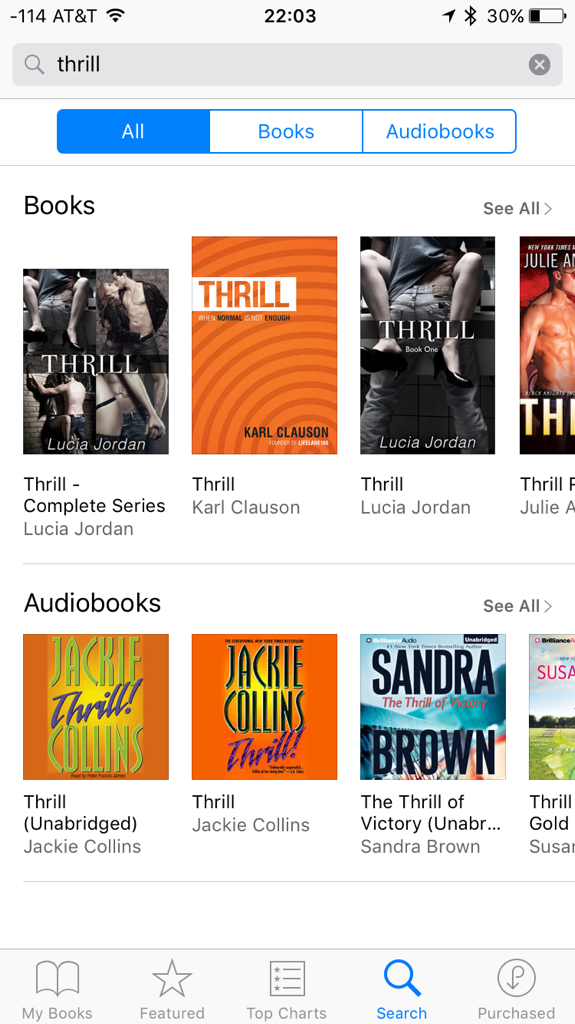
\includegraphics[keepaspectratio, width=3cm]{SearchResults.png}
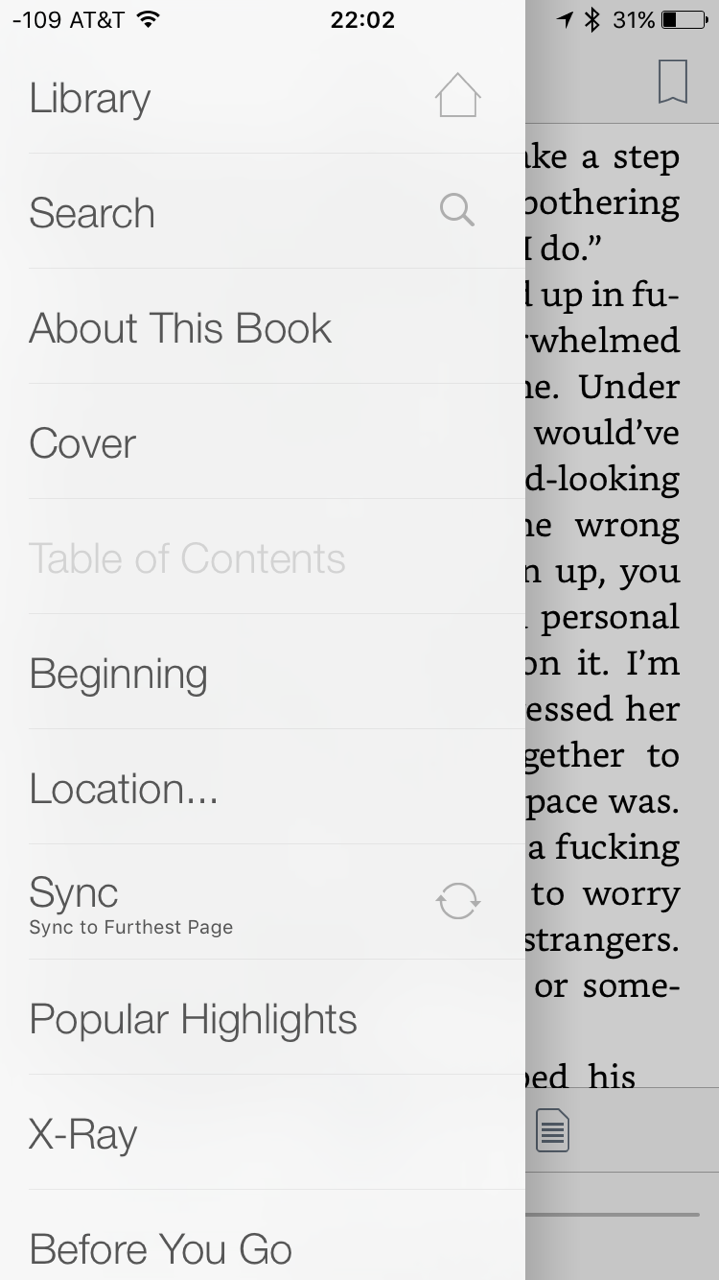
\includegraphics[keepaspectratio, width=3cm]{SearchButton.png}

\section{Analysis}
\subsection{Test 1}
As can be seen from the usability metrics, the Kindle app had less errors than the iBooks app, however in the categories of learnability and satisfaction, iBooks clearly had the upper hand.
\subsubsection{App Inefficiencies}
Learnability for the Kindle app took a hard hit from one of the outliers, who took 125 seconds to perform the task, however having to go through another unrelated application to purchase a book is an inefficiency that the Kindle app introduces. The reason an internet browser is required to make purchases, is because on iOS devices, Apple mandates that in-app purchases be managed by Apple. Amazon, unwilling to comply with this, decided to forgo this option. This is also the cause of much of the negative feedback we got while asking about satisfaction; many people found it silly that they could not purchase books within the Kindle app. In the iBooks application however, when searching for the book title, the desired book was not the first result. The top position was taken by a paid collection of books that make up a series, and the free book that we were looking for showed up second, causing people to hit the top result and thus the wrong book.

\subsection{Test 2}
In Test 2, the tables turned, and the Kindle app took the efficiency, as iBooks had a lengthy outlier. Kindle additionally had less user errors, however apps elicited similarly positive satisfaction responses. Overall, it would seem that in this test, Kindle was the more favorable of the two.
\subsubsection{Operating system influences}
Some of the main difficulties that testers experienced in this test were with things that function differently on different mobile operating systems. Even users who used devices running iOS found this task particularly difficult; one person commented that the highlighting function did not seem to follow the conventions of other iOS applications, which was interesting seeing as iBooks is developed by Apple. The outlier in the iBooks tests is an an avid user of Blackberry devices, where highlighting a selection is done with 2 fingers spanning across the desired passage. On the Kindle side of things, although testers seemed to have an easier time performing the action, they also found it confusing that annotating a selection of text did not automatically highlight it; a feature that one of the testers said was present on the stand alone Kindle devices. However, people generally enjoyed having options as to what color was used to highlight the text.

\subsection{Test 3}
Finally, in test 3, iBooks had a clean sweep across all three categories. In efficiency, not only did Kindle have a large outlier with 80 seconds, even without the outlier included in the average, iBooks took a significant amount of time less than the Kindle app. Additionally, while the iBooks app had an impressive 0 errors, the Kindle app had only 3 users out of the 13 tested get through without an error. These results mirrored the satisfaction comments, where people voiced their displeasure with the search function in the Kindle app.
\subsubsection{Locating desired functions}
This test really evidently displayed the importance of making features easily accessible. The iBooks app displays its search button on the very screen that you are reading on; no need to hit any buttons to show more functions. This made accessing, and subsequently using the search function very easy for users. The Kindle app however caused a lot of issues due to the fact that it does the exact opposite. To reach the search function in the Kindle app, the user has to tap the screen, bringing up the UI (same as on iBooks so far), but then has to tap an unlabeled menu button in the top left, which then displays a drop down menu full of additional features, where you can then find the search function. Adding all these additional hoops to jump through not only slow the process down, but having all these features hidden behind an ambiguous menu button make them much more difficult to find. Many people we tested would hit a wide variety of buttons, and frantically swipe through pages in hopes of eliciting the desired result. Not only this, but users felt like the search function was inferior to that of iBooks, as iBooks had live search results as they typed, while the Kindle search would remain completely unresponsive until the search was actually put through.

\section{Conclusion}
In conclusion, I believe that there are ways that each reading application can improve. I think that Amazon in particular needs to make its application follow more of the conventions held by iOS. This is because so many other apps, both third and first party, specifically try to match the iOS material design. The Kindle app's current design might work well on Android, where apps are more unique, and focus to a lesser degree on matching Android's material design. In addition to this point, Android users are very likely to identify the most problematic button in all 3 tests (the unlabeled menu button in the Kindle app that appears as 3 horizontal stacked lines) as a menu button, whereas this has very little to no presence on iOS. This is because users of the operating system at hand expect certain conventions to be held within apps. However, even the iBooks app slipped up in a few points when it comes to matching Apples design guidelines. Unlabeled buttons stuck out as some of the most common offenders, while the slightly different highlighting method tripped up a couple users. I felt like the Kindle app developers in particular need to be more conscious of which functions would benefit from being readily accessible on the page for a reader to use. In addition, labeling a button that contains a variety of other functions is key to making a smooth user experience.

\end{document}